\documentclass[11pt]{article}
\usepackage[utf8]{inputenc}
\usepackage[czech]{babel}
\usepackage{graphicx}

\title{Krásy počítačové grafiky: Generování bludiště}
\author{Tomáš Maršálek}
\date{9.\, března 2012}

\begin{document}
\maketitle

\section{Zadání}
Napište program v libovolném jazyce, který generuje bludiště a zobrazuje ho na
obrazovce. Vstupem je počet řádků R a sloupců C.

\section{Algoritmus}
Nejpoužívanější způsob vygenerování bludiště je prohledávání do hloubky v
grafu, kde hrany představují zdi bludiště a hrany výsledné kostry reprezentují
probourané zdi. Bez jakýchkoliv úprav ale tento způsob dává příliš zubaté
výsledky. Možným řešením by bylo při výběru směru dalšího postupu
upřednostňovat jeden směr, výsledkem by pak byly dlouhé \uv{chodby} namísto
malých \uv{komůrek}.

Zde je použit jiný algoritmus, který je rovněž založen na hledání kostry grafu.
Je znám jako Primův nebo Jarníkův algoritmus pro hledání nejmenší kostry grafu.
Princip je takřka stejný jako u hledání do hloubky. Hrany grafu odpovídají zdem
v bludišti a navštívené hrany, které ve výsledku tvoří kostru, odpovídají
probouraným zdem. Graf není třeba předgenerovat celý, stačí pro každou nově
objevenou buňku vytvořit nové hrany s náhodnými ohodnoceními.

\section{Implementace}
Program je napsán v jazyce Java SE 6. Vstupem je počet řádků a sloupců.
Výstupem je vykreslené bludiště v okně. Není umožněno interaktivní zacházení s
výsledkem, jedná se pouze o vykreslený obrázek. Bludiště obsahuje právě jednu
možnou cestu k cíli.

Spuštění programu:
\begin{verbatim}
java -jar MazePrim.jar 80 80
\end{verbatim}

\section{Závěr}
Ukázky vygenerovaných bludišť pro oba zmíněné algoritmy.
Zvýrazněné řešení je dotvořeno v programu GIMP použitím plechovky barvy.

\begin{figure}[ht!]
\centering
	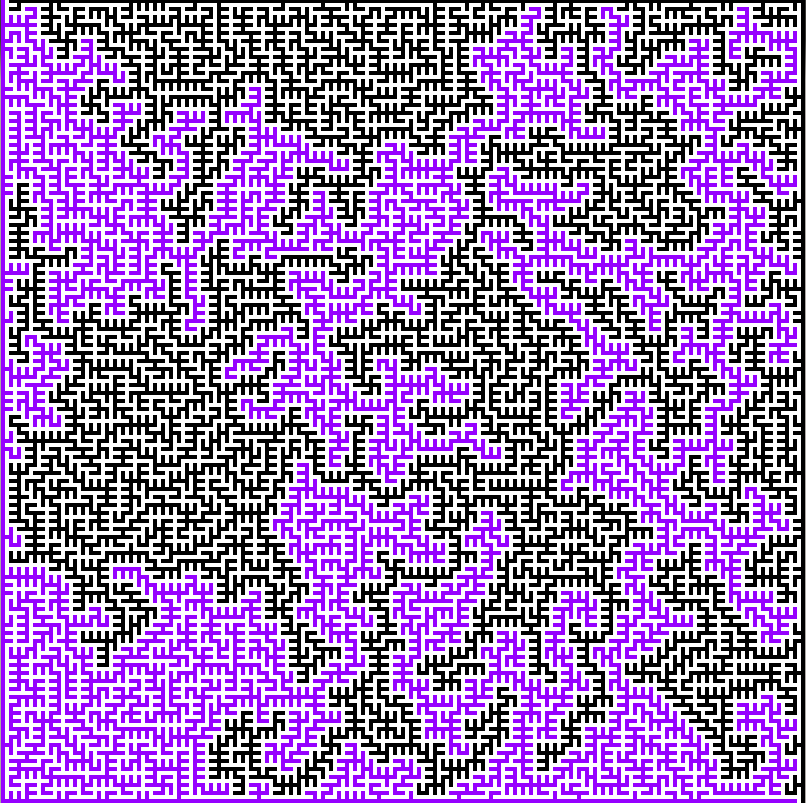
\includegraphics[width=7cm]{dfsmaze.png}
	\caption{Prohledávání do hloubky}
\end{figure}

\begin{figure}[ht!]
\centering
	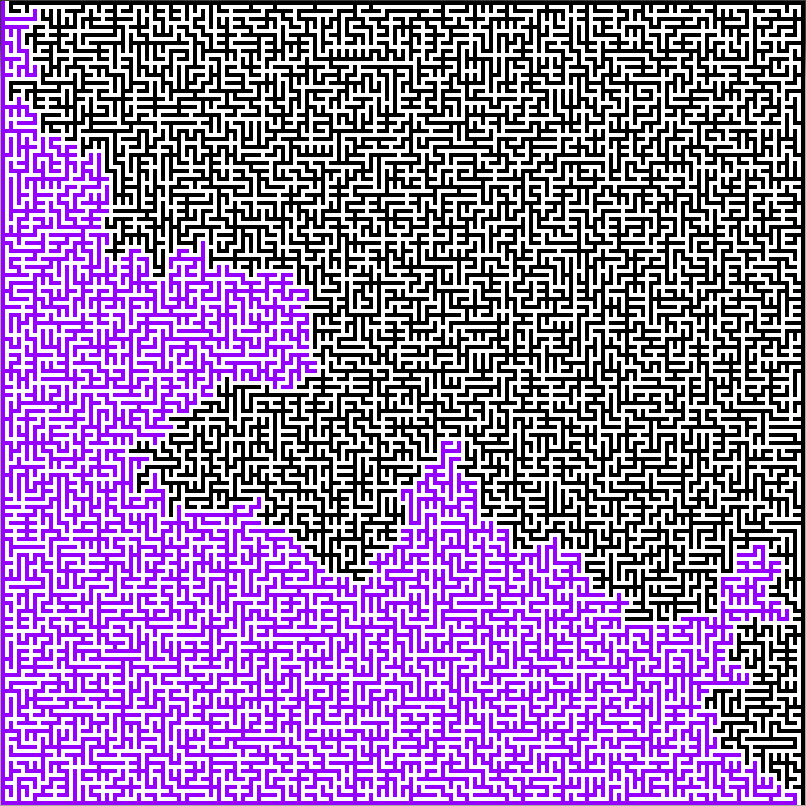
\includegraphics[width=7cm]{primmaze.png}
	\caption{Primův algoritmus}
\end{figure}

\end{document}
